\documentclass[a4paper,12pt]{article}
\usepackage[utf8]{inputenc}
\usepackage[russian]{babel}
\usepackage{amsmath,amssymb}
\usepackage{graphicx}
\usepackage{hyperref}
\usepackage{geometry}
\geometry{top=2cm,bottom=2cm,left=2.5cm,right=2cm}

\begin{document}


% Титульная страница
\begin{titlepage}
	\centering
	\vspace*{1cm}

	{\Huge \textbf{Учебно-методическое пособие по курсу
			\textit{Квантовые вычисления и электроника}}}

	\vspace{0.5cm}
	{\Large для студентов}

	\vspace{1.5cm}

	{\Large Автор: Кандидат физ. мат. наук Эмиль  А. Газазян}

	\vfill

	\vspace{0.8cm}

	{\Large Российско-Армянского университета \\
		Общая физика и квантовые нанострукторы\\
		Ереван\\
		2025}

\end{titlepage}

% Оглавление
\tableofcontents
\newpage

% Введение
\section{Общие сведения о курсе}
\textbf{Название курса:} Квантовые вычисления и электроника\\
%\textbf{Целевая аудитория:} студенты старших курсов бакалавриата или магистратуры (физические, инженерные, ИТ-специальности)\\
%Объём курса: 1 семестр (примерно 16 недель), 2–4 часа занятий в неделю (лекции + практические)\\
\textbf{Форма занятий:} лекции, лабораторные работы/практикумы, групповые проекты, самостоятельная работа\\
\textbf{Основные цели курса:}
Познакомить студентов с основами квантовой механики, лежащими в основе квантовых вычислений.
Изучить принципы построения и функционирования квантовых вычислительных систем.
Рассмотреть основные электронные компоненты, используемые при реализации квантовых систем, а также современные аппаратные платформы.
Провести обзор существующих алгоритмов и программных средств для квантовых вычислений.
Подготовить студентов к дальнейшему изучению квантовой электроники и нанотехнологий.    \\
\textbf{Требования к предварительной подготовке:} базовые знания физики, математики, информатики и электроники.\\


\section{Введение в квантовую механику и квантовые вычисления}
\subsection{История развития квантовой теории}
Первые предпосылки к появлению квантовой теории относятся к концу XIX века. Учёные пытались описать распределение энергии в спектре абсолютно чёрного
тела – задача, которая в то время не имела удовлетворительного решения. Немецкий физик Макс Планк предложил гипотезу, что энергия излучается и поглощается
порциями (квантами) с определённой частотой. Эта гипотеза вошла в историю как «квант планка» и ознаменовала рождение новой физической парадигмы.

Следующим важным шагом стал вклад Альберта Эйнштейна, который интерпретировал фотоны (кванты света) для объяснения фотоэффекта.
Он показал, что свет может вести себя как поток частиц, каждая из которых несёт порцию энергии $E=h\nu$ (где $h$ – постоянная Планка, $\nu$ – частота).
Нильс Бор на основе идей Планка и Эйнштейна разработал планетарную модель атома водорода, в которой электроны могли существовать только на дискретных
энергетических уровнях. Позже Вернер Гейзенберг и Эрвин Шрёдингер независимо друг от друга разработали математические формализмы, ставшие основой квантовой
механики. Гейзенберг использовал матричный подход, а Шрёдингер вывел волновое уравнение, описывающее эволюцию «волновой функции» частицы. Эти взгляды были
объединены Полем Дираком и другими учёными, заложив фундамент современной квантовой теории. В результате сформировалась концепция дуализма «частица–волна»
и появился комплекс ключевых принципов (принцип суперпозиции, принцип неопределённости и др.).
\begin{figure}
	\centering
	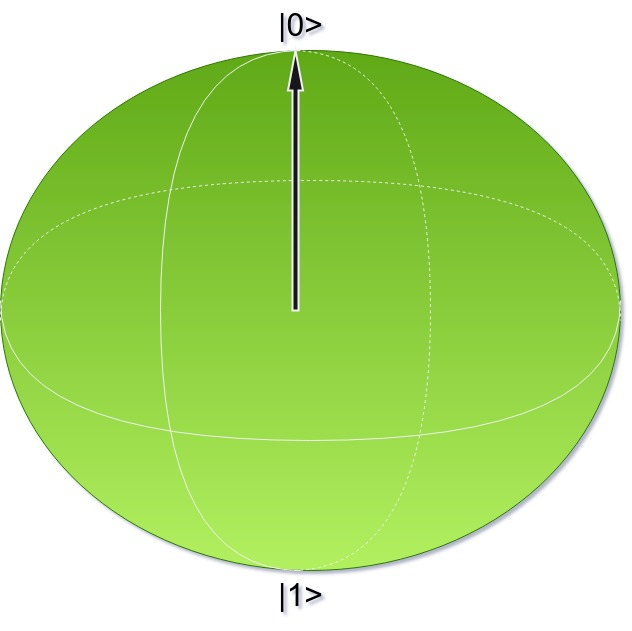
\includegraphics[width=0.3\linewidth]{images/Bloch-Sphere.jpg}
	\caption{Квантовые вычисления}
	\label{fig:Bloch-Sphere}
\end{figure}

\section{Принцип суперпозиции и неопределённости}
\subsection{\textbf{Принцип суперпозиции:}} Согласно принципу суперпозиции, квантовые объекты могут находиться одновременно в нескольких взаимно исключающих
состояниях до тех пор, пока не произведено измерение. Например, классическая частица вроде мяча не может находиться сразу в двух местах, в то время как
микрочастица (электрон, фотон) может описываться суммой нескольких возможных состояний. Эта «сумма» выражается через волновую функцию, которая задаёт
вероятности (амплитуды вероятностей) обнаружить частицу в том или ином состоянии.

Когда мы проводим измерение, волновая функция «коллапсирует» – система «выбирает» одно из состояний в соответствии с вероятностями, заложенными в волновой
функции. До момента измерения система ведёт себя так, словно «пробует» все пути сразу. Этот принцип является одним из наиболее контринтуитивных аспектов
квантовой механики и лежит в основе квантовых вычислений: именно суперпозиция даёт возможность кубиту кодировать больше информации, чем классический бит.

\subsection{\textbf{Принцип  неопределённости:}} Принцип неопределённости Гейзенберга указывает на фундаментальное ограничение при измерении микрочастиц.
Невозможно одновременно с абсолютной точностью знать две сопряжённые величины, например импульс и координату частицы, или энергию и время, отведённое на
измерение. Если мы очень точно замерим положение частицы, то её импульс окажется очень плохо определён, и наоборот.

Этот принцип показывает, что акты измерения необратимо вмешиваются в состояние системы, меняют её и тем самым ограничивают наши возможности в точном
описании микромира. Принцип неопределённости часто считают философским вызовом привычному детерминизму классической физики: в квантовом мире нет полной
предсказуемости – есть лишь вероятности исходов.



\section{Подраздел 2.1}
Другие важные темы или примеры.




\end{document}
